\documentclass[12pt]{beamer}

\usepackage{algorithm}
\usepackage{algorithmic}
\usepackage[english]{babel}
\usepackage{graphicx}
\usepackage[utf8]{inputenc}
\usepackage{tikz}

\usetheme{Copenhagen}
\setbeamertemplate{navigation symbols}{}

\renewcommand{\algorithmiccomment}[1]{/\(\!\)/ #1}

\title{Probability}
\author[Jacopo Notarstefano]{
    Jacopo Notarstefano\\
    \texttt{jacopo.notarstefano [at] gmail.com}
}
\date{11 February 2014}

\begin{document}
    \begin{frame}[plain]
        \titlepage
    \end{frame}

    \begin{frame}{Main ideas}
        \begin{enumerate}
            \item Given two pages, we want to estimate how many pages would be linked
            by both if links were created randomly.
            \item If the actual number is smaller, then we conclude that those pages
            are not related. If it's bigger, we assign a score between \(0\) and \(1\).
            \item This estimate depends on how we model random link creation between
            pages.
        \end{enumerate}
    \end{frame}

    \begin{frame}{The Barabási–Albert model}
        The probability that a new page \(P\) links an existing page \(Q\) is
        proportional to \(\text{indeg}(Q)\): ``The rich get richer''.
        \begin{figure}
            \makebox[\textwidth][c]{
                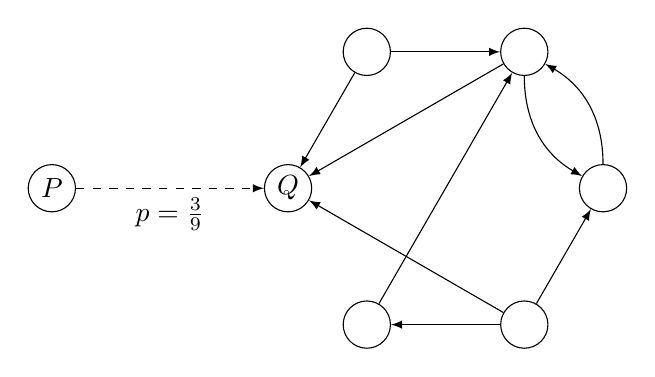
\begin{tikzpicture}
                    \tikzstyle{vertex}=[circle,draw=black!100,inner sep=0pt,minimum size=0.6cm]
                    \node (p) at (1,2) [vertex] {$P$};
                    \node (q) at (4,2) [vertex] {$Q$};
                    \node (v1) at (5,3.732) [vertex] {};
                    \node (v2) at (7,3.732) [vertex] {};
                    \node (v3) at (8,2) [vertex] {};
                    \node (v4) at (7,0.268) [vertex] {};
                    \node (v5) at (5,0.268) [vertex] {};

                    \draw [-latex] (v1) -- (q);
                    \draw [-latex] (v2) -- (q);
                    \draw [-latex] (v4) -- (q);

                    \draw [-latex] (v1) -- (v2);
                    \draw [-latex] (v4) -- (v5);
                    \draw [-latex] (v4) -- (v3);
                    \draw [-latex] (v3) to [in=330,out=90] (v2);
                    \draw [-latex] (v5) -- (v2);
                    \draw [-latex] (v2) to [in=150,out=270] (v3);

                    \draw [-latex,dashed] (p) -- node[below] {\(p = \frac{3}{9}\)} (q);
                \end{tikzpicture}
            }
        \end{figure}
    \end{frame}

    \begin{frame}{Balls and bins, 1/2}
        \begin{problem}
            Suppose that we have \(W\) bins, \(n_1\) red balls and \(n_2\) blue balls.
            When we throw a ball it falls in bin \(i\) with probability \(p_i\). When
            we are done throwing all the balls, what's the expected number of bins with
            both a blue and a red ball?
        \end{problem}
        \begin{figure}
            \makebox[\textwidth][c]{
                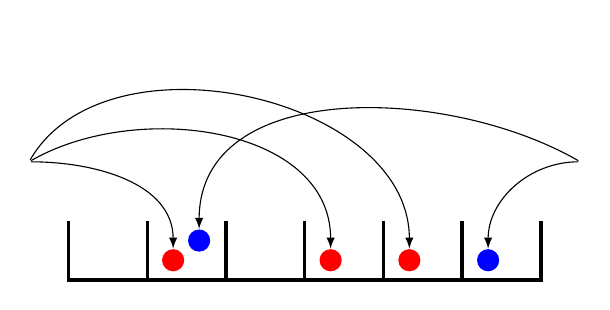
\begin{tikzpicture}
                    \tikzstyle{blue}=[circle,fill=blue!100,inner sep=0pt,minimum size=8pt]
                    \tikzstyle{red}=[circle,fill=red!100,inner sep=0pt,minimum size=8pt]
                    \draw [very thick] (2,0.75) -- (2,0) -- (8,0) -- (8,0.75);
                    \draw [very thick] (3,0.75) -- (3,0);
                    \draw [very thick] (4,0.75) -- (4,0);
                    \draw [very thick] (5,0.75) -- (5,0);
                    \draw [very thick] (6,0.75) -- (6,0);
                    \draw [very thick] (7,0.75) -- (7,0);

                    \node (r1) at (3.33, 0.25) [red] {};
                    \node (r2) at (5.33, 0.25) [red] {};
                    \node (r3) at (6.33, 0.25) [red] {};

                    \node (b1) at (3.66, 0.50) [blue] {};
                    \node (b2) at (7.33, 0.25) [blue] {};

                    \node (r) at (1.5,1.5) [inner sep=0pt] {};
                    \node (b) at (8.5,1.5) [inner sep=0pt] {};

                    \draw [-latex] (r) to [in=90,out=0] (r1);
                    \draw [-latex] (r) to [in=90,out=30] (r2);
                    \draw [-latex] (r) to [in=90,out=60] (r3);
                    
                    \draw [-latex] (b) to [in=90,out=150] (b1);
                    \draw [-latex] (b) to [in=90,out=180] (b2);
                \end{tikzpicture}
            }
        \end{figure}
    \end{frame}

    \begin{frame}{Balls and bins, 2/2}
        \begin{solution}
            If \textbf{all throws are independent}, then, by linearity of expectation,
            we have
            \[
                \mathrm{E}[\vert N_1\cap N_2\vert] = \sum_{i,j=1}^{n_1,n_2}{\mathrm{E}[I_{ij}]} = n_{1}n_{2}\sum_{i=1}^{W}{p_{i}^2} = n_{1}n_{2}\mathbf{P}
            \]
            where \(I_{ij}\) is random indicator variable denoting that red ball \(i\)
            and blue ball \(j\) landed in the same bin.
        \end{solution}
    \end{frame}

    \begin{frame}{The algorithm}
        \begin{algorithm}[H]
            \caption{Probability}
            \begin{algorithmic}[]
                \STATE \, \COMMENT Preprocessing step
                \STATE Scan Wikipedia and compute \(\mathbf{P}\)
                \STATE \, \COMMENT For each pair of pages \(P_1\) and \(P_2\)
                \STATE \(N_{1} \leftarrow \text{outLinks}(P_1)\); \(n_{1} \leftarrow N_{1}.\text{length}\)
                \STATE \(N_{2} \leftarrow \text{outLinks}(P_2)\); \(n_{2} \leftarrow N_{2}.\text{length}\)
                \STATE \(\text{actualValue} \leftarrow \vert N_{1}\cap N_{2}\vert\)
                \STATE \(\text{expectedValue} \leftarrow n_{1}n_{2}\cdot \mathbf{P}\)
                \IF{\(\text{actualValue} < \text{expectedValue}\)}
                    \RETURN \(0\)
                \ELSE
                    \RETURN \(\text{normalize}(actualValue - expectedValue)\)
                \ENDIF
            \end{algorithmic}
        \end{algorithm}
    \end{frame}

    \begin{frame}{Results}
        The algorithm manages to retain the recall baseline while improving on its
        precision, thus achieving a better F1 score.
        \begin{figure}
            \makebox[\textwidth][c]{
                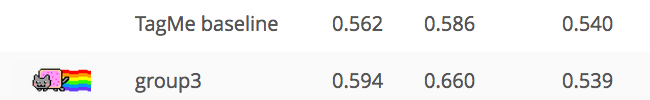
\includegraphics[scale=0.35]{tex/img/nyan}
            }
        \end{figure}

        The algorithm is also fast: a run against the entire AIDA/CoNLL dataset
        takes less than \(2\) minutes.
    \end{frame}
\end{document}
